\documentclass[border=6pt,tikz]{standalone}
\usepackage{tikz}
\usepackage{amsmath,amssymb}
\usetikzlibrary{arrows.meta,positioning,fit,backgrounds,calc,shapes.geometric,decorations.pathreplacing,patterns}
\definecolor{ink}{HTML}{1B2430}
\definecolor{muted}{HTML}{6B7785}
\definecolor{accent}{HTML}{2F6FB5}
\definecolor{accent2}{HTML}{C1611F}
\definecolor{good}{HTML}{2E7D5B}
\definecolor{soft}{HTML}{EDF2F7}
\definecolor{soft2}{HTML}{FBEDE2}
\definecolor{soft3}{HTML}{E6F0E9}
\tikzset{
  box/.style={draw=ink,line width=.7pt,rounded corners=2pt,fill=soft,inner sep=4pt,align=center,font=\sffamily\small},
  boxa/.style={box,fill=soft2},
  boxb/.style={box,fill=soft3},
  plain/.style={align=center,font=\sffamily\small,text=ink},
  tiny/.style={align=center,font=\sffamily\scriptsize,text=muted},
  ar/.style={-{Stealth[length=2.4mm]},draw=ink,line width=.7pt},
  arm/.style={-{Stealth[length=2.4mm]},draw=muted,line width=.6pt,dashed},
  nd/.style={circle,draw=ink,line width=.7pt,fill=white,minimum size=7mm,inner sep=0pt,font=\sffamily\scriptsize},
  ndf/.style={nd,fill=soft},
  ndt/.style={nd,fill=soft2},
}

\begin{document}
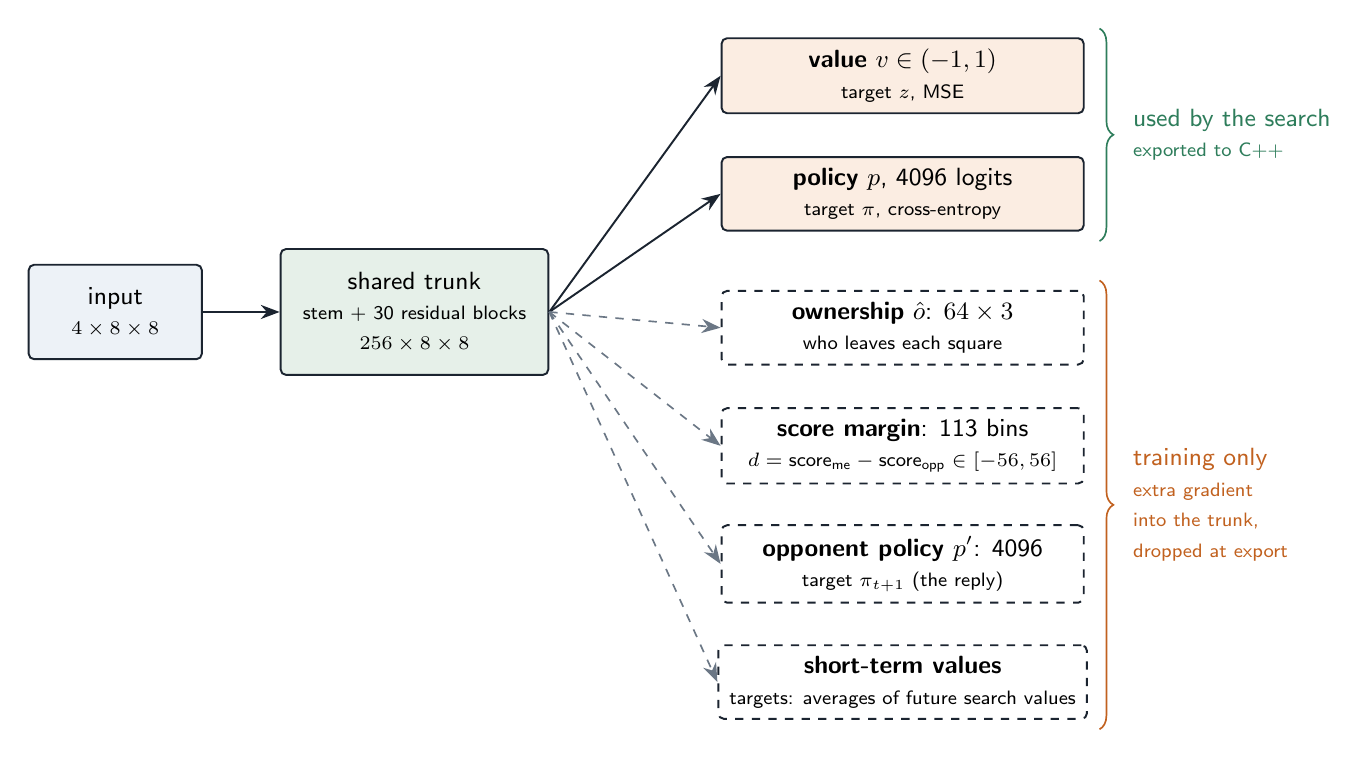
\begin{tikzpicture}[x=1mm,y=1mm]
  \node[box,minimum width=22mm,minimum height=12mm] (in) at (0,0) {input\\\scriptsize $4\times8\times8$};
  \node[boxb,minimum width=34mm,minimum height=16mm] (trunk) at (38,0) {shared trunk\\\scriptsize stem + 30 residual blocks\\\scriptsize $256\times8\times8$};
  \draw[ar] (in) -- (trunk);
  % existing heads
  \node[boxa,minimum width=46mm] (v) at (100,30) {\textbf{value} $v\in(-1,1)$\\\scriptsize target $z$, MSE};
  \node[boxa,minimum width=46mm] (p) at (100,15) {\textbf{policy} $p$, 4096 logits\\\scriptsize target $\pi$, cross-entropy};
  % auxiliary heads
  \tikzset{aux/.style={box,dashed,fill=white,minimum width=46mm}}
  \node[aux] (own) at (100,-2) {\textbf{ownership} $\hat o$: $64\times3$\\\scriptsize who leaves each square};
  \node[aux] (sc) at (100,-17) {\textbf{score margin}: 113 bins\\\scriptsize $d=\text{score}_{\text{me}}-\text{score}_{\text{opp}}\in[-56,56]$};
  \node[aux] (op) at (100,-32) {\textbf{opponent policy} $p'$: 4096\\\scriptsize target $\pi_{t+1}$ (the reply)};
  \node[aux] (st) at (100,-47) {\textbf{short-term values}\\\scriptsize targets: averages of future search values};
  \foreach \h in {v,p} \draw[ar] (trunk.east) -- (\h.west);
  \foreach \h in {own,sc,op,st} \draw[arm] (trunk.east) -- (\h.west);
  \draw[decorate,decoration={brace,amplitude=5pt},line width=.6pt,draw=good] (125,36) -- (125,9) node[midway,right=3mm,plain,text=good,align=left]{used by the search\\\scriptsize exported to C++};
  \draw[decorate,decoration={brace,amplitude=5pt},line width=.6pt,draw=accent2] (125,4) -- (125,-53) node[midway,right=3mm,plain,text=accent2,align=left]{training only\\\scriptsize extra gradient\\\scriptsize into the trunk,\\\scriptsize dropped at export};
\end{tikzpicture}
\end{document}
